\section{Theorie}
Das Ziel dieses Versuches ist es, die Kristallstruktur und die Größe der Einheitszelle
von zwei verschiedenen Probematerialien zu bestimmen, indem Debye-Scherrer-Aufnahmen
angefertigt werden.

\subsection{Beschreibung von Kristallstrukturen}
Ein Großteil der kondesierten Materie liegt in kristalliner Struktur vor.
Um dieser Struktur aufzulösen, muss die räumliche Auflösung des Messgeräts in der
gleichen Größenordnung liegen wie die Abstände zwischen den Atomen. Dafür eignen sich
neben langsamen Neutronen oder Elektronen auch Röntgenstrahlen. Die im folgenden
beschriebene Methode basiert auf der Beugung dieser Röntgenstrahlung an der Kristallstruktur.

Die räumliche Beschreibung der Kristalle lässt sich aus zwei Elementen zusammensetzen:
der Basis und des Punktgitters. Zusammen ergeben sie die Kristallstruktur, wie in
\autoref{abb:struktur} dargestellt.
\begin{figure}
  \centering
  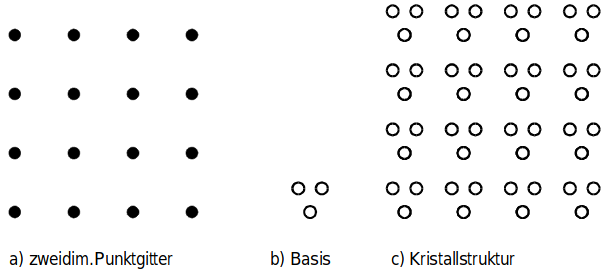
\includegraphics[scale=0.5]{content/pics/basis_gitter.png}
  \caption{Bestandteile der Kristallstruktur. \cite{anleitung}}
  \label{abb:struktur}
\end{figure}

\section{Durchführung}
\subsection{Aufbau}
\subsection{Versuchsdurchführung}
